\documentclass[11pt]{report}
\usepackage{amsmath}
\usepackage{amssymb}
\usepackage{graphicx}
\usepackage{tikz}



\begin{document}
	
	\begin{figure}
		\centering
		\begin{tikzpicture}
			\draw[thick, ->] (0,-3)--(0,5);
			\draw[thick, ->] (-3,0)--(5,0);
			\node at (1.8,-.28){$a$};
			%%%%%%%%%%%%%%%%%%%%%%%%%%%%%%%%
			\draw[thick] (0,0)--(3,4.5)--(3,0);
			\node at (1,2){$r$};
			\node at (3.4,2){$b$};
			\node at (3.2,4.5){$z$};
			%%%%%%%%%%%%%%%%%%%%%%%%%%%%%
			\draw (.7,0) arc(0:65:6mm);
			\node at(1,0.4){$\theta$};
		\end{tikzpicture}\caption{Trigonometric Form of a Complex Number}\label{fig:1_3_1}
	\end{figure}

	\begin{figure}
		\centering
		\begin{tikzpicture}
			\draw[thick, ->] (0,-0.5)--(0,5);
			\draw[thick, ->] (-.5,0)--(5.3,0);
			\node at (2.8,-.5){$x$};
			\node at (-0.3, -0.3){0};
			%%%%%%%%%%%%%%%%%%%%%%%%%%%%%%%%
			\draw[dashed] (0,4.5)--(4.3,4.5)--(4.3,4.5)--(4.3,0);
			%%%%%%%%%%%%%%%%%%%%%%%%%%%%%
			\draw[dashed] (0,0)--(4.3,4.5);
			\node at (1.5,2){$r$};
			\node at (4.6,2){$y$};
			\draw (.9,0) arc(0:65:6mm);
			\node at(1.1,0.4){$\theta$};
		\end{tikzpicture}\caption{Polar Form of a Complex Number}\label{fig:1_4_1}
	\end{figure}

	\begin{figure}
		\centering
		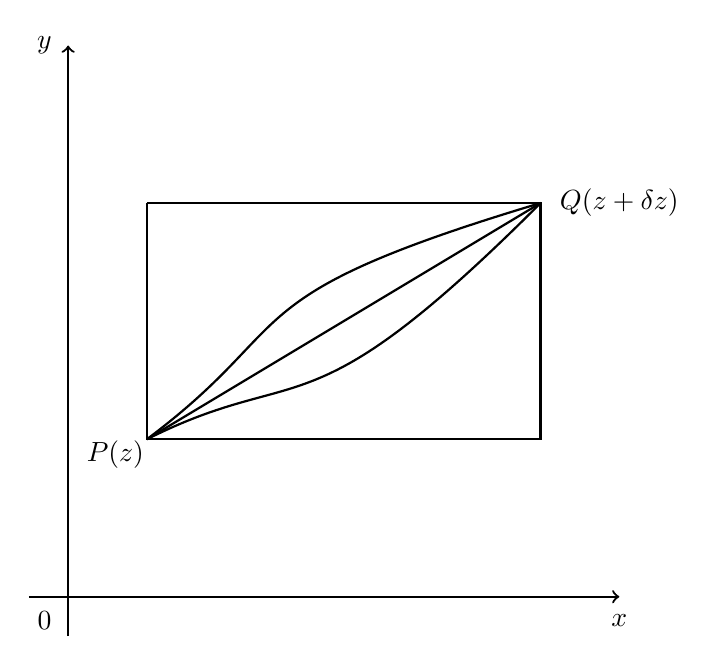
\begin{tikzpicture}
			\draw[thick, ->] (0,-0.5)--(0,7);
			\draw[thick, ->] (-.5,0)--(7,0);
			\node at (7,-.3){$x$};
			\node at (-0.3,7){$y$};
			\node at (-0.3, -0.3){0};
			%%%%%%%%%%%%%%%%%%%%%%%%%%%%%%%%
			\draw[thick] (1,5)--(6,5)--(6,2)--(1,2)--(1,5);
			\node at (.6,1.8){$P(z)$};
			\node at (7,5){$Q(z+\delta z)$};
			%%%%%%%%%%%%%%%%%%%%%%%%%%%%%
			\draw[thick] (1,2) -- (6,5);
			\draw[thick] (1,2) .. controls (3,3.5) and (2,3.8) .. (6,5);
			\draw[thick] (1,2) .. controls (3,3) and (3,2) .. (6,5);
		\end{tikzpicture}\caption{}\label{fig:_}
	\end{figure}

\end{document}